\section{Shannon's Theorem}

Following from our previous discussion, we can see that this is the challenge we face in Coding Theory; how do we balance reliability with efficiency? Is it possible to create a perfectly balanced code?. In communication systems, engineers had the belief that errors during transmission were inevitable, that at most we can minimize the rate of error. Keep in mind this is not speaking in terms of the previously mentioned error probability $p$, rather, the error rate in this case is the difference between the original message and the final decoded message. The main question posed was: 'Is it possible to reliably transmit information over noisy channels, and if so, how quickly?'.

This is where we would like to introduce the notion of \textit{capacity}. But before this we must build an understanding of what are \textit{information} and \textit{entropy}. \\

\subsection{Information}
In information theory, the amount of information we get from an event is defined as 

\begin{equation}
    I(X = x) = \log( \frac{1}{P(x)} )
    \label{eq:info}
\end{equation}


where $P(x)$ is the probability of event $x$. This quantity can be though of intuitively as the 'surprise factor'; how surprised are you of this outcome? Trivially, if the probability of an event is almost certain, your surprise factor would be 0 and vice versa as observed in $I$. The base of the log determines the unit, either nats for base $e$ or bits for base 2. For our context, we will be using base 2 hereafter. \\

\subsection{Entropy}
\textbf{Entropy} of a random variable is defined as

\begin{equation}
\label{eqn:entropy}
    H(X) = \sum_{x \in X}{P(X=x)\log\left( \frac{1}{P(X=x)} \right)}
\end{equation}


Comparing this with the way we obtain the average of a random variable below:
\[\mu_{x} = \sum x \cdot P(x)\] \\

It can be intuitively understood that Entropy is the average information you get from a random variable. The more distributed the probability function, the greater the average information. It can also be thought of non-mathematically as the \emph{randomness}. \\

In the case of a BSC, the plot of entropy to probability is seen in Figure \ref{fig:entropyplot}.

\begin{figure}
    \centering
    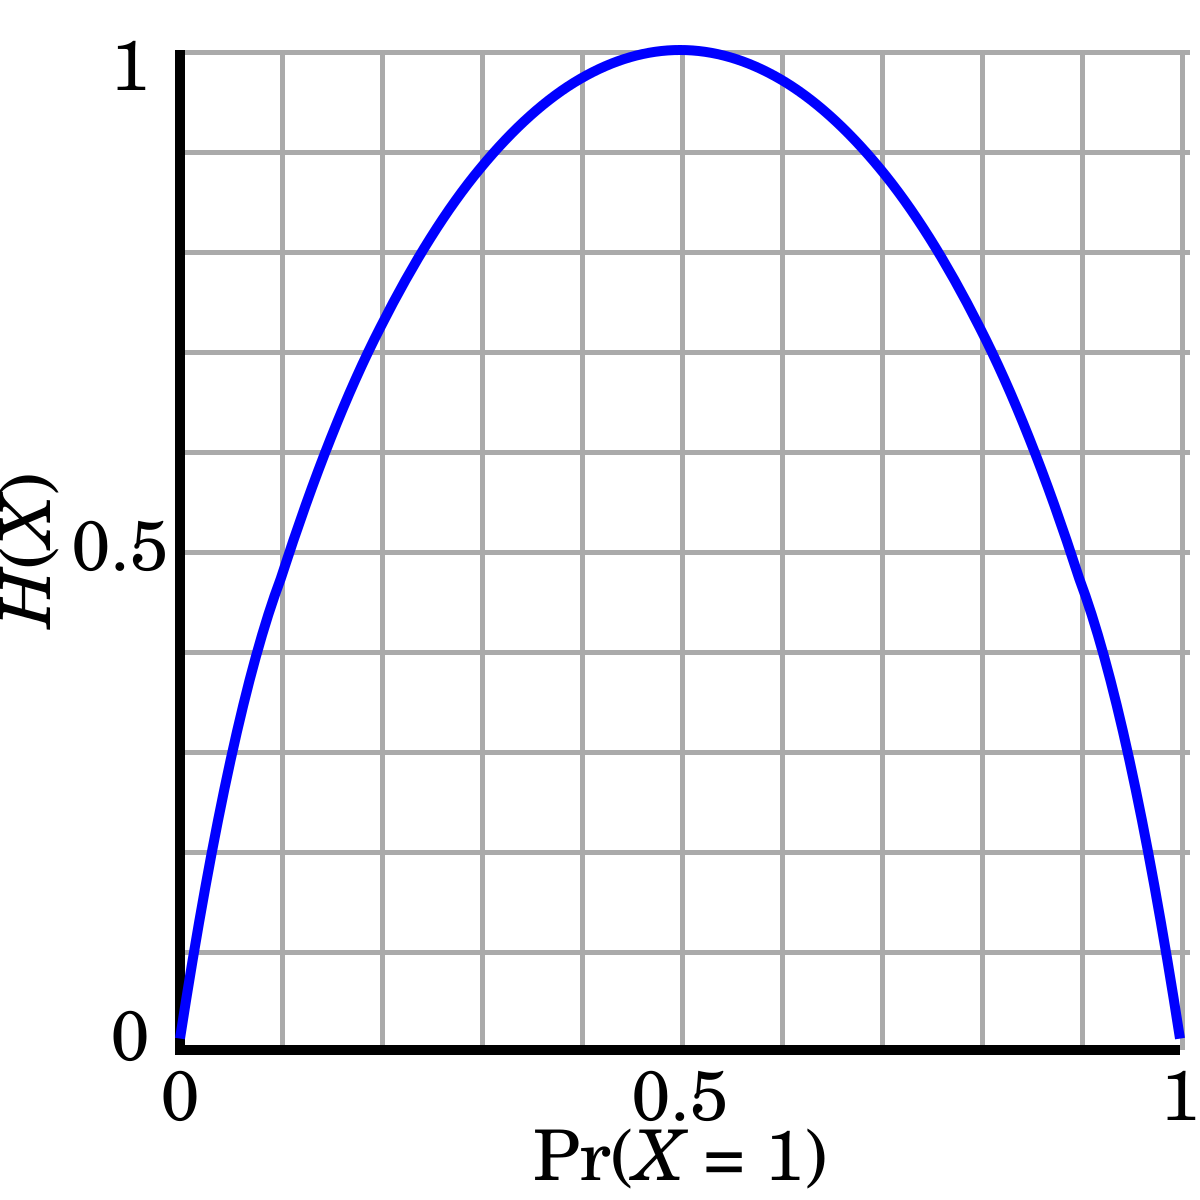
\includegraphics[width=0.5\linewidth]{images/entropyplot.png}
    \caption{Entropy of a BSC}
    \label{fig:entropyplot}
\end{figure}

For example, say you flip a  fair coin once. The two events are:
\[
P(H) = 0.5, \quad P(T) = 0.5
\]

The entropy is:
\[
H(X) = - \big[ 0.5 \log_2 0.5 + 0.5 \log_2 0.5 \big]
= - \big[ 0.5(-1) + 0.5(-1) \big]
= 1 \; \text{bit}.
\]

Thus, each fair coin toss carries exactly $1$ bit of information.

If the coin is biased, say
\[
P(H) = 0.9, \quad P(T) = 0.1,
\]
then the entropy is:
\[
H(X) = - \big[ 0.9 \log_2 0.9 + 0.1 \log_2 0.1 \big]
\approx 0.47 \; \text{bits}.
\]

So, the biased coin has less uncertainty, hence lower entropy. \\

\subsection{Mutual Information}
An abstract concept following naturally from entropy is mutual information or 'how much more information do I have about random variable X if I am given Y if they depend on eachother'. Mutual information is denoted: 
\begin{equation}
    I(X;Y) = H(X) - H(X|Y)
   \label{eq:info}
\end{equation}
 

Where $H(X|Y)$ is defined as:

\begin{equation}
    H(X \mid Y) = - \sum_{y \in \mathcal{Y}} P(y) 
   \sum_{x \in \mathcal{X}} P(x \mid y) \, \log_2 P(x \mid y).
   \label{eq:conditionalentropy}
\end{equation}



\subsubsection{Example with Perfect Dependence}
An example will provide you with better insight and intuition on mutual information.

Consider again the fair coin toss $X$ from the previous example regarding entropy.
Let
\[
X = \text{Toss of a fair coin (H/T)}, 
\quad 
Y = \text{``Is the coin heads?'' (Yes/No)}.
\]

If you know $X$, then you know $Y$. If you know $Y$, you also know $X$.

The entropies are:
\[
H(X) = 1 \;\text{bit}, 
\quad 
H(Y) = 1 \;\text{bit}.
\]

The conditional entropy is:
\[
H(Y \mid X) = 0.
\]
because given X, you already know Y with certainty.

Therefore, the mutual information is:
\[
I(X;Y) = H(Y) - H(Y \mid X) = 1 - 0 = 1 \;\text{bit}.
\]

This means if you measure X, you get 1 bit of information about Y and vice versa.
\\


A nice visual of entropy in terms of a venn diagram is available in Figure \ref{fig:entropy}.

\begin{figure}
    \centering
    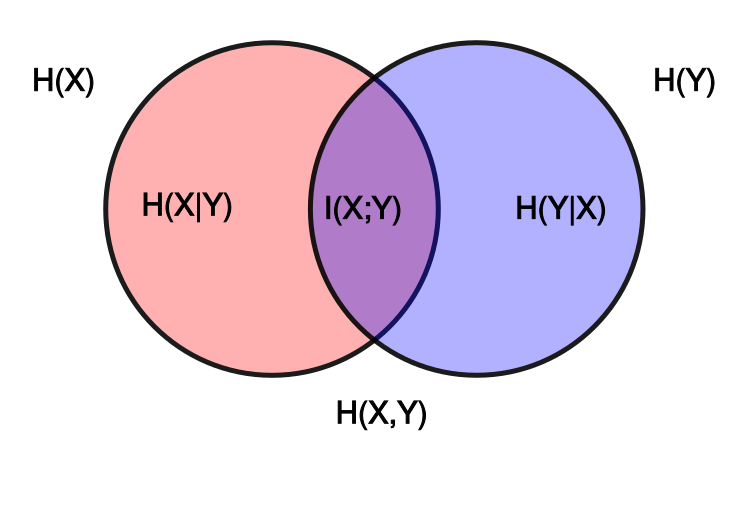
\includegraphics[width=0.5\linewidth]{images/entropy.png}
    \caption{Venn diagram representation of entropy and information}
    \label{fig:entropy}
\end{figure}


\subsection{Capacity}

The abstract definition of capacity follows from the idea of mutual information. \\

\textbf{Definition 8:} Capacity is the maximum amount of information transmitted per channel use. Mathematically, it is the maximum mutual information we have on sent message x given received message y: $max \ \ I(X;Y)$ \\

In 1948, Claude Shannon wrote the theorem relating channel capacity with the information rate of a channel, proving that it is possible to have completely error-free communication in discrete memoryless channels so long as the information rate $R < C$ where $C$ is the 'channel capacity'. \\

\textbf{Theorem 1.1:} $\forall$ binary symmetric channels with $0 \le p < \frac{1}{2}$, $\exists$ channel capacity $C$ s.t all codewords ${\mathbf{x}}$ can always be reliably decoded into their original message $\mathbf{u}$ with arbitrarily low error probability $Pr_{e}$ so long as $R < C$.  \\

 In the case of binary symmetric channels, maximum capacity is defined as: $C = 1 - H(p) = 1 + p\log_{2}{p} + (1-p)\log_{2}{(1-p)}$ .$Pr_{e}$ tends to at most $2^{-\sigma n}$.  where $\sigma = 1-H(p) -R$, aka the difference between maximum and actual rate So as $n \to \infty$, the error rate approaches 0. \\

However, one may ask, won't the error rate approach 0 regardless of the value of R? This is a question I thought to myself and the answer is very clearly no. Assume $R > C$, then $\sigma < 0$, and so $Pr_{e}$ would diverge as n increases. And so the converse of the theorem is presented where, in the case $R>C$, reliable communication is impossible. 
\\
While Shannon's theorem was revolutionary, it unfortunately did not provide an empirical method to creating such efficient codes. However, by knowing this limit, engineers and mathematicians alike were able to evaluate and design their codes to be as efficient as possible while still being reliable. Examples of this include Turbo Codes (1993), LDPC codes (1990), and now Polar Codes (2008). \\

To feed our curiosity, let us present a very brief overview of the strategy of a geometric proof to feed the reader's curiosity and provide a general intuitive understanding. This proof is for the case of binary symmetric channels. \\


Take a randomly generated linear code \textbf{C} with some encoding and decoding function. Efficiency does not matter. Our decoding function will be minimum distance decoding. Let's return to our hamming space visualization in \ref{fig:ball2} and recall our explanation of error as the \textit{drift} of the output within its respective hamming ball. By the law of large numbers, the received codeword is almost surely going to be within $pn$ distance of the original codeword. 

The number of possible sequences with exactly $pn$ flips using Stirling's approximation is \[
\binom{n}{pn} \approx 2^{nH(p)}.
\] 

Since the total number of binary sequences of length \(n\) is \(2^n\), the maximum number of disjoint Hamming balls you can pack is approximately
\[
\frac{2^n}{2^{nH(p)}} = 2^{n(1-H(p))}.
\]

This shows that reliable communication is possible only if the code rate satisfies
\[
R < 1 - H(p).
\]
